% =====================================================================
%  Manual del usuario · Analista Académico v4
%  Compilar con:  ./construir_manual.sh   (o: latexmk -pdf manual_usuario.tex)
%  Navegación: marcadores del PDF, índice y mapa rápido con enlaces, enlaces en la
%  cabecera de cada página, índice local por capítulo, barra anterior/siguiente
%  y referencias cruzadas entre secciones.
% =====================================================================
\documentclass[11pt,letterpaper,oneside]{report}

\usepackage[utf8]{inputenc}
\usepackage[T1]{fontenc}
\usepackage{lmodern}
\usepackage[spanish,es-noshorthands,es-tabla,es-nodecimaldot]{babel}
\usepackage[margin=2.2cm,top=2.7cm,bottom=2.4cm,headheight=16pt,headsep=12pt]{geometry}
\usepackage{xcolor}
\usepackage{graphicx}
\usepackage{tabularx}
\usepackage{booktabs}
\usepackage{longtable}
\usepackage{array}
\usepackage{enumitem}
\usepackage{fancyhdr}
\usepackage{titlesec}
\usepackage{amsmath}
\usepackage{float}
\usepackage{caption}
\usepackage{lastpage}
\usepackage{tikz}
\usetikzlibrary{positioning,arrows.meta,shapes.geometric}
\usepackage[most]{tcolorbox}
\usepackage{fontawesome5}
\usepackage{etoc}
\usepackage{etoolbox}
\usepackage[
  unicode,
  colorlinks=true,
  linkcolor=primario,
  urlcolor=azul,
  citecolor=primario,
  bookmarksnumbered=true,
  bookmarksopen=true,
  bookmarksopenlevel=0,
  pdfpagemode=UseOutlines,
  pdfstartview=FitH,
  pdfdisplaydoctitle=true,
  pdftitle={Manual del usuario - Analista Académico},
  pdfsubject={Análisis de notas por competencias de uno o varios grupos},
  pdfkeywords={competencias, notas, analítico, práctico, pensamiento crítico, informes}
]{hyperref}
\usepackage{bookmark}

% ---------------------------------------------------------------- Colores
\definecolor{primario}{HTML}{4F46E5}
\definecolor{primariooscuro}{HTML}{3730A3}
\definecolor{violeta}{HTML}{6D28D9}
\definecolor{fondo}{HTML}{EEF2FF}
\definecolor{azul}{HTML}{2563EB}
\definecolor{analitico}{HTML}{2563EB}
\definecolor{practico}{HTML}{059669}
\definecolor{critico}{HTML}{9333EA}
\definecolor{verde}{HTML}{047857}
\definecolor{ambar}{HTML}{B45309}
\definecolor{rojo}{HTML}{B91C1C}
\definecolor{gris}{HTML}{4B5563}
\definecolor{grisclaro}{HTML}{F3F4F6}

\setlength{\parindent}{0pt}
\setlength{\parskip}{6pt}
\renewcommand{\familydefault}{\sfdefault}
\captionsetup{font={small,it},labelfont={bf,color=primario}}
\setlist{itemsep=2pt,topsep=4pt}

% ---------------------------------------------------------------- Títulos
\newcommand{\capitulotitulo}[1]{%
  \begin{tcolorbox}[enhanced,colback=primario,colframe=primario,coltext=white,arc=4pt,
     boxsep=8pt,left=10pt,interior style={left color=primario,right color=violeta}]
  \ifnum\value{chapter}>0 {\large\bfseries Capítulo \thechapter}\\[2pt]\fi
  {\Huge\bfseries #1}
  \end{tcolorbox}}
\titleformat{\chapter}[block]{\normalfont\sffamily}{}{0pt}{\capitulotitulo}
\titlespacing*{\chapter}{0pt}{-20pt}{6pt}
\titleformat{\section}{\normalfont\sffamily\Large\bfseries\color{primario}}{\thesection}{0.6em}{}[{\color{primario!30}\titlerule[0.8pt]}]
\titleformat{\subsection}{\normalfont\sffamily\large\bfseries\color{primariooscuro}}{\thesubsection}{0.6em}{}
\titlespacing*{\section}{0pt}{14pt}{6pt}

% ---------------------------------------------------------------- Cabecera y pie con enlaces
\pagestyle{fancy}
\fancyhf{}
\renewcommand{\headrulewidth}{0.4pt}
\renewcommand{\headrule}{\hbox to\headwidth{\color{primario!40}\leaders\hrule height \headrulewidth\hfill}}
\fancyhead[L]{\small\sffamily\hyperref[mapa]{\faMap\ Mapa rápido}\quad\hyperref[indice]{\faListUl\ Índice}}
\fancyhead[C]{\small\sffamily\color{gris}\nouppercase{\leftmark}}
\fancyhead[R]{\small\sffamily\hyperref[cap:glosario]{\faBook\ Glosario}\quad\hyperref[cap:problemas]{\faQuestionCircle\ Ayuda}}
\fancyfoot[L]{\footnotesize\sffamily\color{gris}Analista Académico v4 · Manual del usuario}
\fancyfoot[R]{\footnotesize\sffamily\color{gris}Página \thepage\ de \pageref*{LastPage}}
\fancypagestyle{plain}{}  % las páginas de capítulo usan la misma cabecera con enlaces
\renewcommand{\chaptermark}[1]{\markboth{\ifnum\value{chapter}>0 \thechapter.\ \fi#1}{}}

% ---------------------------------------------------------------- Comandos de navegación
% Botón con enlace a una etiqueta
\newcommand{\boton}[3][primario]{\hyperref[#2]{\tcbox[on line,colback=#1,colframe=#1,coltext=white,
  boxsep=1pt,left=5pt,right=5pt,top=2pt,bottom=2pt,arc=3pt,fontupper=\sffamily\small\bfseries]{#3}}}
% Enlace a una sección mostrando su número y nombre: \ver{sec:etiqueta}
\newcommand{\ver}[1]{\hyperref[#1]{\faArrowCircleRight\,\ref*{#1}~\nameref*{#1}}}
% Enlace a una pestaña de la aplicación
\newcommand{\pest}[2]{\hyperref[#1]{\textbf{\faWindowMaximize\,#2}}}
% Texto de un botón o campo de la interfaz
\newcommand{\ui}[1]{\tcbox[on line,colback=grisclaro,colframe=gris!40,boxrule=0.4pt,boxsep=0pt,left=3pt,right=3pt,top=1pt,bottom=1pt,arc=2pt]{\sffamily\small #1}}
% Nombre de una columna del archivo
\newcommand{\col}[1]{\texttt{\small #1}}
% Etiquetas de carácter
\newcommand{\dimA}{\textcolor{analitico}{\textbf{Analítico}}}
\newcommand{\dimP}{\textcolor{practico}{\textbf{Práctico}}}
\newcommand{\dimC}{\textcolor{critico}{\textbf{Pensamiento crítico}}}

% Índice local al comienzo de cada capítulo
\newcommand{\enestecapitulo}{%
  \etocsettocstyle{\begin{tcolorbox}[enhanced,colback=fondo,colframe=primario!35,arc=3pt,
      title={\faListUl\ En este capítulo (haga clic para ir)},fonttitle=\sffamily\bfseries\small,
      colbacktitle=primario!80,coltitle=white,left=6pt,right=6pt,top=2pt,bottom=2pt]\small}{\end{tcolorbox}}%
  \etocsetnexttocdepth{section}%
  \localtableofcontents}

% Barra de navegación al final de cada capítulo: \navegacion{anterior}{siguiente}
\newcommand{\navegacion}[2]{%
  \par\vspace{10pt}\noindent
  \begin{tcolorbox}[enhanced,colback=grisclaro,colframe=gris!25,arc=3pt,boxsep=3pt,left=4pt,right=4pt]
  \ifx&#1&\else\boton{#1}{\faChevronLeft\ \nameref*{#1}}\fi\hfill
  \boton[gris]{mapa}{\faMap\ Mapa}\ \boton[gris]{indice}{\faListUl\ Índice}\hfill
  \ifx&#2&\else\boton{#2}{\nameref*{#2}\ \faChevronRight}\fi
  \end{tcolorbox}}

% Cuadros de consejo, atención, nota y "ver también"
\newtcolorbox{consejo}{enhanced,colback=practico!7,colframe=practico,boxrule=0pt,leftrule=3pt,arc=0pt,
  left=8pt,fontupper=\small,before upper={\textcolor{practico}{\faLightbulb\ \textbf{Consejo.}}\ }}
\newtcolorbox{atencion}{enhanced,colback=ambar!8,colframe=ambar,boxrule=0pt,leftrule=3pt,arc=0pt,
  left=8pt,fontupper=\small,before upper={\textcolor{ambar}{\faExclamationTriangle\ \textbf{Atención.}}\ }}
\newtcolorbox{nota}{enhanced,colback=fondo,colframe=primario,boxrule=0pt,leftrule=3pt,arc=0pt,
  left=8pt,fontupper=\small,before upper={\textcolor{primario}{\faInfoCircle\ \textbf{Nota.}}\ }}
\newtcolorbox{vertambien}{enhanced,colback=white,colframe=primario!30,boxrule=0.5pt,arc=3pt,
  left=8pt,fontupper=\small,before upper={\textcolor{primario}{\faLink\ \textbf{Ver también:}}\ }}

% Pasos numerados
\newlist{pasos}{enumerate}{1}
\setlist[pasos]{label={\tcbox[on line,colback=primario,colframe=primario,coltext=white,boxsep=0pt,left=3pt,right=3pt,top=1pt,bottom=1pt,arc=6pt,fontupper=\sffamily\scriptsize\bfseries]{\arabic*}},leftmargin=2.2em,itemsep=4pt}

% Captura de pantalla: \captura[ancho]{archivo}{pie}{etiqueta}
\newcommand{\captura}[4][0.96\linewidth]{%
  \begin{figure}[H]\centering
  {\setlength{\fboxsep}{0pt}\fcolorbox{gris!35}{white}{\includegraphics[width=#1]{img/#2}}}
  \caption{#3}\label{fig:#4}
  \end{figure}}

\graphicspath{{./}}

% Más espacio para los números de dos cifras en el índice
\makeatletter
\patchcmd{\l@chapter}{1.5em}{2.3em}{}{}
\renewcommand*\l@section{\@dottedtocline{1}{2.3em}{2.9em}}
\makeatother

% =====================================================================
\begin{document}

% ---------------------------------------------------------------- Portada
\thispagestyle{empty}
\pdfbookmark[0]{Portada}{portada}
\phantomsection\label{portada}
\begin{tikzpicture}[remember picture,overlay]
  \shade[left color=primario,right color=violeta] (current page.north west) rectangle ([yshift=-9.5cm]current page.north east);
  \node[anchor=north west,text=white,font=\sffamily\bfseries\fontsize{34}{40}\selectfont,align=left]
    at ([xshift=2.2cm,yshift=-3cm]current page.north west) {Analista Académico};
  \node[anchor=north west,text=white,font=\sffamily\LARGE,align=left]
    at ([xshift=2.2cm,yshift=-4.9cm]current page.north west) {Manual del usuario · versión 4};
  \node[anchor=north west,text=white!85!primario,font=\sffamily\large,align=left,text width=16cm]
    at ([xshift=2.2cm,yshift=-6.3cm]current page.north west)
    {Análisis de notas por competencias de uno o varios grupos:\\ analítico, práctico y pensamiento crítico.};
\end{tikzpicture}
\vspace*{8.4cm}

\begin{tcolorbox}[enhanced,colback=fondo,colframe=primario,arc=4pt,title={\faCompass\ Cómo moverse por este manual},
  fonttitle=\sffamily\bfseries,colbacktitle=primario,left=8pt,right=8pt]
Todo lo que aparece en \textcolor{primario}{\textbf{este color}} es un enlace: haga clic para ir.
\begin{itemize}[leftmargin=1.4em]
  \item \textbf{Mapa rápido}: una página con botones a cada tema y a las tareas más frecuentes.
  \item \textbf{Índice}: todos los capítulos y secciones con su página.
  \item \textbf{Cabecera de cada página}: enlaces a \emph{Mapa rápido}, \emph{Índice}, \emph{Glosario} y \emph{Ayuda} (solución de problemas).
  \item \textbf{Inicio de cada capítulo}: un recuadro «En este capítulo» con enlaces a sus secciones.
  \item \textbf{Final de cada capítulo}: botones para ir al capítulo anterior o al siguiente.
  \item \textbf{Marcadores del PDF}: el panel lateral del lector muestra el contenido completo.
  \item Dentro de la aplicación, el botón \ui{? Ayuda} abre este manual en la parte que explica la pestaña en la que usted está.
\end{itemize}
\end{tcolorbox}

\vspace{6pt}
\begin{center}
\boton{mapa}{\faMap\ Ir al mapa rápido}\quad
\boton{indice}{\faListUl\ Ir al índice}\quad
\boton{tarea:ungrupo}{\faPlayCircle\ Empezar: primer análisis}\quad
\boton{cap:problemas}{\faQuestionCircle\ Tengo un problema}
\end{center}

\vfill
{\small\color{gris} Fecha de esta edición: 7 de octubre de 2026. La aplicación funciona en el navegador abriendo \texttt{index.html}; no necesita instalación.}
\clearpage

% ---------------------------------------------------------------- Mapa rápido
\chapter*{Mapa rápido}
\phantomsection\label{mapa}
\addcontentsline{toc}{chapter}{Mapa rápido}
\markboth{Mapa rápido}{}
\vspace*{-12pt}
\textbf{Flujo de trabajo.} Haga clic en cada paso para ir a su explicación.

\begin{center}
\begin{tikzpicture}[
  paso/.style={rectangle,rounded corners=4pt,draw=primario,fill=fondo,thick,minimum width=2.55cm,minimum height=1.2cm,align=center,font=\sffamily\small},
  flecha/.style={-{Stealth[length=3mm]},thick,primario}]
  \node[paso] (a) {\hyperref[cap:archivos]{\textbf{0. Archivos}}\\[1pt]{\scriptsize notas y competencias}};
  \node[paso,right=0.35cm of a] (b) {\hyperref[cap:datos]{\textbf{1. Datos}}\\[1pt]{\scriptsize cargar grupos}};
  \node[paso,right=0.35cm of b] (c) {\hyperref[cap:evaluaciones]{\textbf{2. Evaluaciones}}\\[1pt]{\scriptsize pesos y carácter}};
  \node[paso,right=0.35cm of c] (d) {\hyperref[cap:analisis]{\textbf{3. Análisis}}\\[1pt]{\scriptsize del grupo}};
  \node[paso,below=0.4cm of d] (e) {\hyperref[cap:estudiantes]{\textbf{4. Estudiantes}}\\[1pt]{\scriptsize filtros y fichas}};
  \node[paso,left=0.35cm of e] (f) {\hyperref[cap:informes]{\textbf{5. Informes}}\\[1pt]{\scriptsize PDF y Excel}};
  \node[paso,left=0.35cm of f,draw=critico,fill=critico!8] (g) {\hyperref[cap:programa]{\textbf{6. Programa}}\\[1pt]{\scriptsize todos los grupos}};
  \node[paso,left=0.35cm of g,draw=practico,fill=practico!8] (h) {\hyperref[cap:respaldo]{\textbf{Guardar}}\\[1pt]{\scriptsize respaldo .json}};
  \draw[flecha] (a) -- (b); \draw[flecha] (b) -- (c); \draw[flecha] (c) -- (d);
  \draw[flecha] (d) -- (e); \draw[flecha] (e) -- (f); \draw[flecha] (f) -- (g); \draw[flecha] (g) -- (h);
\end{tikzpicture}
\end{center}

\textbf{Temas del manual.}

\begin{tcbraster}[raster columns=2,raster equal height=rows,raster column skip=8pt,raster row skip=4pt,
  enhanced,colback=white,colframe=primario!35,arc=3pt,fonttitle=\sffamily\bfseries\small,colbacktitle=fondo,coltitle=primariooscuro,
  left=5pt,right=5pt,top=3pt,bottom=3pt,fontupper=\footnotesize]
\begin{tcolorbox}[title={\hyperref[cap:intro]{\faHome\ 1. Introducción y conceptos}}]
\hyperref[sec:conceptos]{Conceptos clave} · \hyperref[sec:flujo]{Flujo recomendado} · \hyperref[sec:cabecera]{Cabecera y pestañas}
\end{tcolorbox}
\begin{tcolorbox}[title={\hyperref[cap:archivos]{\faFileExcel\ 2. Preparar los archivos}}]
\hyperref[sec:planilla]{Planilla de notas} · \hyperref[sec:variosgrupos]{Varios grupos} · \hyperref[sec:csv]{CSV} · \hyperref[sec:catalogo]{Catálogo de competencias}
\end{tcolorbox}
\begin{tcolorbox}[title={\hyperref[cap:datos]{\faFolderOpen\ 3. Pestaña 1 · Datos}}]
\hyperref[sec:cargarnotas]{Cargar planillas} · \hyperref[sec:listagrupos]{Grupo activo} · \hyperref[sec:cargarcatalogo]{Catálogo} · \hyperref[sec:escala]{Escala y niveles}
\end{tcolorbox}
\begin{tcolorbox}[title={\hyperref[cap:evaluaciones]{\faTasks\ 4. Pestaña 2 · Evaluaciones}}]
\hyperref[sec:pesos]{Porcentajes} · \hyperref[sec:asociar]{Competencias} · \hyperref[sec:caracterev]{Carácter} · \hyperref[sec:recursos]{Recursos} · \hyperref[sec:copiar]{Copiar a grupos}
\end{tcolorbox}
\begin{tcolorbox}[title={\hyperref[cap:analisis]{\faChartBar\ 5. Pestaña 3 · Análisis del grupo}}]
\hyperref[sec:kpis]{Indicadores} · \hyperref[sec:dimgrupo]{Por carácter} · \hyperref[sec:estadisticas]{Estadísticas} · \hyperref[sec:alertas]{Alertas}
\end{tcolorbox}
\begin{tcolorbox}[title={\hyperref[cap:estudiantes]{\faUserGraduate\ 6. Pestaña 4 · Estudiantes}}]
\hyperref[sec:rapidos]{Filtros rápidos} · \hyperref[sec:criterios]{Criterios Y/O} · \hyperref[sec:ficha]{Ficha y observaciones}
\end{tcolorbox}
\begin{tcolorbox}[title={\hyperref[cap:informes]{\faFilePdf\ 7. Pestaña 5 · Informes}}]
\hyperref[sec:tiposinf]{Tipos} · \hyperref[sec:opcionesinf]{Opciones} · \hyperref[sec:contenidoinf]{Contenido} · \hyperref[sec:exportar]{PDF, Excel, impresión}
\end{tcolorbox}
\begin{tcolorbox}[title={\hyperref[cap:programa]{\faUniversity\ 8. Pestaña 6 · Programa}}]
\hyperref[sec:dimprog]{Carácter global} · \hyperref[sec:hallazgos]{Hallazgos} · \hyperref[sec:comparativo]{Comparativo} · \hyperref[sec:riesgoprog]{Riesgo}
\end{tcolorbox}
\begin{tcolorbox}[title={\hyperref[cap:caracter]{\faBrain\ 9. Carácter de las competencias}}]
\hyperref[sec:clasificacion]{Clasificación} · \hyperref[sec:corregir]{Corregir} · \hyperref[sec:dimnota]{Nota por carácter} · \hyperref[sec:interpretar]{Interpretar}
\end{tcolorbox}
\begin{tcolorbox}[title={\hyperref[cap:calculos]{\faCalculator\ 10. Cómo se calcula}}]
\hyperref[sec:formulas]{Fórmulas} · \hyperref[sec:estados]{Estados} · \hyperref[sec:niveles]{Niveles} · \hyperref[sec:indprog]{Programa}
\end{tcolorbox}
\begin{tcolorbox}[title={\hyperref[cap:respaldo]{\faSave\ 11. Guardar y respaldos}}]
\hyperref[sec:autoguardado]{Guardado automático} · \hyperref[sec:respaldo]{Respaldo} · \hyperref[sec:nuevo]{Empezar de nuevo}
\end{tcolorbox}
\begin{tcolorbox}[title={\hyperref[cap:manual]{\faBookOpen\ 12. Pestaña 7 · Manual y ayuda}}]
Índice lateral, búsqueda de temas y botón \emph{Ayuda} de cada pestaña.
\end{tcolorbox}
\end{tcbraster}

\textbf{¿Qué quiere hacer?}

\begin{tcbraster}[raster columns=3,raster equal height,raster column skip=6pt,raster row skip=4pt,enhanced,
  colback=practico!6,colframe=practico!50,arc=3pt,fontupper=\footnotesize\sffamily,left=4pt,right=4pt,top=3pt,bottom=3pt]
\begin{tcolorbox}\hyperref[tarea:ungrupo]{\faPlayCircle\ Analizar un grupo por primera vez}\end{tcolorbox}
\begin{tcolorbox}\hyperref[tarea:varios]{\faUsers\ Analizar varios grupos del programa}\end{tcolorbox}
\begin{tcolorbox}\hyperref[tarea:riesgo]{\faExclamationTriangle\ Informes para estudiantes en riesgo}\end{tcolorbox}
\begin{tcolorbox}\hyperref[tarea:coordinacion]{\faUniversity\ Informe para coordinación o comité}\end{tcolorbox}
\begin{tcolorbox}\hyperref[tarea:critico]{\faBrain\ Fortalecer el pensamiento crítico}\end{tcolorbox}
\begin{tcolorbox}\hyperref[tarea:actualizar]{\faRedo\ Actualizar notas a mitad del semestre}\end{tcolorbox}
\end{tcbraster}

\clearpage
% ---------------------------------------------------------------- Índice
\phantomsection\label{indice}
\pdfbookmark[0]{Índice}{indice}
\etocsettocstyle{\chapter*{Índice}\markboth{Índice}{}}{}
\etocsetnexttocdepth{section}
\tableofcontents
\clearpage

% =====================================================================
\chapter{Introducción}\label{cap:intro}
\enestecapitulo

\section{¿Qué hace la aplicación?}\label{sec:quehace}
\textbf{Analista Académico} lee las planillas de notas de sus grupos (Excel o CSV) y el catálogo de competencias de sus cursos, y le ayuda a:
\begin{itemize}
  \item calcular para cada estudiante la nota acumulada, el promedio, la nota que necesita en lo que falta y su estado (aprobando, en riesgo, ya no alcanza…), ver \ver{sec:formulas};
  \item saber qué competencias debe reforzar cada estudiante y qué recursos de estudio recomendarle;
  \item medir el desempeño en tres \textbf{caracteres} de las competencias: \dimA, \dimP\ y \dimC, ver \ver{cap:caracter};
  \item filtrar estudiantes con varios criterios a la vez y escribir observaciones;
  \item comparar varios grupos del mismo programa y obtener hallazgos y recomendaciones automáticas, ver \ver{cap:programa};
  \item generar informes en PDF (individual, del grupo y del programa) y consolidados en Excel.
\end{itemize}

\section{Requisitos y cómo abrirla}\label{sec:requisitos}
\begin{itemize}
  \item Un navegador actualizado: Chrome, Edge, Firefox o Safari.
  \item Abra el archivo \texttt{index.html} de la carpeta de la aplicación (doble clic). No requiere instalación ni servidor.
  \item La primera vez necesita conexión a internet para descargar las librerías que leen Excel y crean PDF. Si no hay conexión, la aplicación lo avisa, ver \ver{cap:problemas}.
  \item Los datos se quedan en su computador: no se envían a ningún servidor, ver \ver{sec:privacidad}.
\end{itemize}

\section{Conceptos clave}\label{sec:conceptos}
\begin{description}[style=nextline,leftmargin=1.2em,font=\color{primario}\bfseries]
  \item[Grupo] Un conjunto de estudiantes con su planilla de notas. Puede venir de un archivo, de una hoja o de un valor de la columna \col{Grupo}, ver \ver{sec:variosgrupos}.
  \item[Grupo activo] El grupo con el que trabajan las pestañas 2 a 5. Se elige en la cabecera, ver \ver{sec:listagrupos}.
  \item[Programa] El conjunto de todos los grupos cargados. Se analiza en la pestaña 6, ver \ver{cap:programa}.
  \item[Evaluación] Cada columna de notas (parcial, quiz, taller…). Tiene un porcentaje (peso) en la nota final.
  \item[Evaluación pendiente] Una evaluación que nadie del grupo ha presentado todavía (la columna está vacía).
  \item[Competencia] Lo que el estudiante debe saber hacer, con su criterio de evaluación; viene del catálogo, ver \ver{sec:catalogo}.
  \item[Carácter] La dimensión de una competencia: \dimA, \dimP\ o \dimC, ver \ver{sec:tresdim}.
  \item[Logro] El porcentaje de estudiantes que alcanzan la nota aprobatoria en una competencia o en un carácter.
\end{description}
En el \hyperref[cap:glosario]{\faBook\ Glosario} encontrará todos los términos con enlaces a su explicación.

\section{Flujo de trabajo recomendado}\label{sec:flujo}
\begin{pasos}
  \item Prepare la planilla de notas y el catálogo de competencias (\ver{cap:archivos}).
  \item En \pest{cap:datos}{1. Datos} cargue las planillas de uno o varios grupos y el catálogo; elija el curso de cada grupo.
  \item En \pest{cap:evaluaciones}{2. Evaluaciones} revise porcentajes, fechas, competencias y carácter de cada evaluación.
  \item Revise el \pest{cap:analisis}{3. Análisis del grupo} y la lista de \pest{cap:estudiantes}{4. Estudiantes}.
  \item Genere los \pest{cap:informes}{5. Informes} para estudiantes, acudientes o coordinación.
  \item Si tiene varios grupos, consulte el análisis del \pest{cap:programa}{6. Programa}.
  \item Guarde un respaldo (\ver{sec:respaldo}).
\end{pasos}

\section{La cabecera y las pestañas}\label{sec:cabecera}
\captura{cabecera.jpg}{Cabecera de la aplicación: selector del grupo activo, botones de respaldo, \emph{Nuevo}, \emph{Ayuda} y las pestañas.}{cabecera}
\begin{itemize}
  \item \textbf{Subtítulo}: asignatura, grupo, periodo y docente del grupo activo.
  \item \ui{Grupo activo}: aparece cuando hay dos o más grupos; cambia el grupo que muestran las pestañas 2 a 5.
  \item \ui{Guardar respaldo} y \ui{Abrir respaldo}: ver \ver{sec:respaldo}. \ui{Nuevo}: ver \ver{sec:nuevo}.
  \item \ui{? Ayuda}: abre la pestaña 7 en la página de este manual que explica la pestaña actual, ver \ver{cap:manual}.
  \item Los números junto a las pestañas indican cuántas evaluaciones, estudiantes y grupos hay.
\end{itemize}

\navegacion{}{cap:archivos}

% =====================================================================
\chapter{Preparar los archivos}\label{cap:archivos}
\enestecapitulo

\section{Planilla de notas}\label{sec:planilla}
Una fila por estudiante. La aplicación lee \textbf{todas} las columnas y las clasifica por su encabezado y por su contenido:

\begin{longtable}{>{\raggedright\arraybackslash}p{3.6cm}>{\raggedright\arraybackslash}p{6.2cm}>{\raggedright\arraybackslash}p{5.6cm}}
\toprule
\textbf{Tipo de columna} & \textbf{Encabezados reconocidos} & \textbf{Uso}\\\midrule\endhead
Nombre (obligatoria) & \col{Nombres y Apellidos}, \col{Estudiante}, \col{Alumno}, o \col{Nombres} y \col{Apellidos} separadas & Nombre en tablas e informes.\\
Documento & \col{ID}, \col{Documento}, \col{Código}, \col{Cédula}, \col{TI}… & Identifica al estudiante. Si se repite, se agrega un sufijo y se avisa.\\
Parciales & \col{1P}, \col{2P}, \col{Parcial 1}, \col{2do parcial} & Evaluación de tipo parcial.\\
Quices & \col{Q1}, \col{Quiz 2} & Evaluación de tipo quiz.\\
Otras evaluaciones & \col{Taller 1}, \col{Seguimiento}, \col{Proyecto}, \col{Examen final}, \col{Laboratorio} & Evaluación del tipo correspondiente.\\
Grupo y asignatura & \col{Grupo}, \col{Sección}, \col{Paralelo}, \col{NRC}; \col{Asignatura}, \col{Materia}, \col{Curso} & Dividen la hoja en grupos, ver \ver{sec:variosgrupos}.\\
Docente & \col{Docente}, \col{Profesor} & Docente del grupo.\\
Informativas & \col{DF}, \col{Definitiva}, \col{Faltas}, \col{Inasistencias}; columnas con valores fuera de la escala & Se muestran como referencia; \textbf{no} entran en la nota.\\
Texto por estudiante & \col{Observaciones}, \col{Competencias}, \col{Páginas web}, \col{Videos}, \col{Ejercicios}, \col{Herramientas} & Observaciones y recomendaciones personales en el informe.\\
\bottomrule
\end{longtable}

\begin{consejo}
Deje \textbf{vacías} las evaluaciones que aún no se han hecho: la aplicación las toma como \emph{pendientes} y calcula cuánto necesita cada estudiante en ellas. Escriba \col{NP} cuando un estudiante no presentó una evaluación que el grupo sí presentó.
\end{consejo}
\begin{atencion}
Una nota fuera de la escala (por ejemplo 11 en una escala de 0 a 5) o un texto en una columna de notas se deja vacío y se informa en «Observaciones de la lectura», ver \ver{sec:cargarnotas}.
\end{atencion}

\section{Varios grupos}\label{sec:variosgrupos}
Puede analizar varios grupos a la vez de tres maneras (y combinarlas):
\begin{enumerate}
  \item \textbf{Un archivo por grupo}: seleccione o arrastre varios archivos juntos.
  \item \textbf{Un archivo con una hoja por grupo}: cada hoja con columna de nombres es un grupo.
  \item \textbf{Una sola hoja con columna \col{Grupo}} (y opcionalmente \col{Asignatura} y \col{Docente}): la hoja se divide en un grupo por cada valor distinto, por ejemplo «Cálculo Diferencial · 01» y «Cálculo Diferencial · 02».
\end{enumerate}
Cuando vuelve a cargar el mismo archivo, sus grupos se \textbf{actualizan} (no se duplican) y conservan los porcentajes, fechas, competencias y observaciones.

\section{Archivos CSV}\label{sec:csv}
\begin{itemize}
  \item Se aceptan archivos \texttt{.csv} (y \texttt{.txt}) separados por coma, punto y coma o tabulación; el separador se detecta solo.
  \item Con punto y coma se acepta la coma decimal (\texttt{3,5}).
  \item Los textos con el separador dentro van entre comillas: \texttt{"Bien; atento"}.
  \item Se reconocen los CSV guardados por Excel en español (Windows-1252) y en UTF-8: las tildes se leen bien.
  \item La carpeta \texttt{ejemplos} trae \texttt{ejemplo\_dos\_grupos.csv} para probar.
\end{itemize}

\section{Catálogo de competencias}\label{sec:catalogo}
Un libro de Excel con \textbf{una hoja por curso}. Cada hoja tiene las columnas \col{Competencias} (\texttt{1. Texto de la competencia…}) y \col{Criterios de Evaluación}. Columnas opcionales \col{Páginas web}, \col{Videos}, \col{Ejercicios} y \col{Herramientas} se usan como recursos de cada competencia.
\begin{itemize}
  \item Las filas sin número al final de la hoja se guardan como \emph{notas del curso}.
  \item Excel recorta los nombres de hoja a 31 caracteres; puede corregir el nombre del curso en la aplicación, ver \ver{sec:cargarcatalogo}.
  \item El verbo con que empieza cada competencia define su carácter automático, ver \ver{sec:clasificacion}. Redáctelas empezando por el verbo: «Analizar…», «Aplicar…», «Justificar…».
\end{itemize}

\section{Plantilla y datos de ejemplo}\label{sec:plantilla}
En la pestaña 1, \ui{Descargar plantilla de notas} entrega un Excel con las columnas recomendadas, un catálogo de ejemplo y las instrucciones. \ui{Cargar datos de ejemplo} crea tres grupos de Cálculo Diferencial (60 estudiantes) para conocer la aplicación sin sus archivos.

\navegacion{cap:intro}{cap:datos}

% =====================================================================
\chapter{Pestaña 1 · Datos}\label{cap:datos}
\enestecapitulo

\section{Cargar las planillas de notas}\label{sec:cargarnotas}
\begin{pasos}
  \item Haga clic en el recuadro \ui{Seleccione o arrastre uno o varios archivos Excel o CSV}, o arrastre los archivos sobre él.
  \item Puede elegir varios archivos a la vez (tecla \texttt{Ctrl} o \texttt{Shift} en el selector).
  \item Al terminar, un mensaje indica cuántos grupos y estudiantes se cargaron.
\end{pasos}
\captura[0.52\linewidth]{datos_notas.jpg}{Planillas de notas: zona de carga, lista de grupos y resumen del grupo activo.}{datosnotas}
Debajo de la lista de grupos aparece el resumen del \textbf{grupo activo}:
\begin{itemize}
  \item \textbf{Evaluaciones}: los chips con borde punteado son evaluaciones \emph{pendientes}.
  \item \textbf{Otras columnas leídas}: informativas (definitiva, faltas) y de texto (observaciones, recursos).
  \item \textbf{Observaciones de la lectura}: avisos sobre notas fuera de escala, documentos repetidos, estudiantes sin notas, etc.
\end{itemize}

\section{Lista de grupos y grupo activo}\label{sec:listagrupos}
Cada fila de la lista es un grupo:
\begin{itemize}
  \item \textbf{Nombre}: se puede cambiar escribiendo en el campo (por ejemplo «Mateunov0» $\rightarrow$ «Matemáticas I · G1»).
  \item \textbf{Origen}: archivo, hoja y valor de la columna \col{Grupo}.
  \item \textbf{Est.}: número de estudiantes.
  \item \textbf{Curso de competencias}: el curso del catálogo que corresponde a ese grupo.
  \item \ui{Activar}: convierte ese grupo en el grupo activo. El grupo activo tiene la etiqueta \textcolor{verde}{\textbf{Activo}}.
  \item \ui{\textcolor{rojo}{x}}: quita el grupo (pide confirmación).
\end{itemize}
\begin{nota}
El grupo activo también se cambia con el selector \ui{Grupo activo} de la cabecera (\ver{sec:cabecera}) o haciendo clic en un grupo en la pestaña 6 (\ver{sec:comparativo}).
\end{nota}

\section{Cargar el catálogo de competencias}\label{sec:cargarcatalogo}
\captura[0.52\linewidth]{datos_competencias.jpg}{Catálogo de competencias del grupo activo, con el carácter de cada una.}{datoscomp}
\begin{itemize}
  \item El catálogo es \textbf{común a todos los grupos}. Se carga una vez.
  \item \ui{Curso del grupo activo}: elija el curso. Si el grupo no tenía competencias asociadas, se reparten automáticamente entre sus evaluaciones (\ver{sec:asociar}).
  \item \ui{Nombre del curso}: corríjalo si Excel lo recortó.
  \item Los chips de colores muestran cuántas competencias del curso son \dimA, \dimP\ y \dimC.
  \item \ui{Usar este curso en todos los grupos}: asigna el mismo curso a los demás grupos.
  \item \ui{Revisar el carácter de las competencias}: abre la ventana de corrección, ver \ver{sec:corregir}.
\end{itemize}
\begin{atencion}
Si el nombre del archivo no permite adivinar el curso, la aplicación propone el primero del catálogo. Revise el curso de cada grupo en la lista de grupos.
\end{atencion}

\section{Datos del grupo}\label{sec:datosgrupo}
\captura[0.6\linewidth]{datos_curso.jpg}{Datos que aparecen en el encabezado de los informes.}{datoscurso}
\textbf{Institución}, \textbf{programa} y \textbf{periodo} se aplican a todos los grupos. \textbf{Asignatura}, \textbf{grupo}, \textbf{docente} y \textbf{correo} son de cada grupo. Si el nombre del grupo era el automático, se actualiza al cambiar la asignatura o el grupo.

\section{Escala, criterios y niveles}\label{sec:escala}
\captura[0.6\linewidth]{datos_escala.jpg}{Escala de calificación, criterios y niveles de desempeño (se aplican a todos los grupos).}{datosescala}
\begin{itemize}
  \item \textbf{Nota mínima, máxima y aprobatoria} (por defecto 0, 5 y 3) y número de \textbf{decimales}.
  \item \ui{Una celda vacía en una evaluación ya calificada cuenta como 0}: si está marcada, quien no presentó una evaluación que el grupo sí presentó recibe 0. Si se desmarca, esa evaluación no cuenta para ese estudiante. Ver \ver{sec:pendientes}.
  \item \ui{Riesgo alto si necesita más de}: umbral para el estado «Riesgo alto» (por defecto 4.0), ver \ver{sec:estados}.
  \item \textbf{Niveles de desempeño}: nombre y nota desde la cual aplica cada nivel, ver \ver{sec:niveles}.
\end{itemize}

\navegacion{cap:archivos}{cap:evaluaciones}

% =====================================================================
\chapter{Pestaña 2 · Evaluaciones y competencias}\label{cap:evaluaciones}
\enestecapitulo

\section{La tabla de evaluaciones}\label{sec:tablaev}
\captura{evaluaciones.jpg}{Evaluaciones del grupo activo con porcentaje, competencias, carácter y recursos.}{evaluaciones}
\begin{tabularx}{\linewidth}{>{\bfseries}l X}
\toprule
Incluir & Si se desmarca, la evaluación no entra en la nota.\\
Evaluación & Nombre que aparece en los informes (editable).\\
Columna & Encabezado original en el archivo.\\
Tipo & Parcial, quiz, taller, seguimiento, proyecto, examen final u otra.\\
Fecha & Fecha de la evaluación (aparece en el informe individual).\\
Peso (\%) & Porcentaje de la nota final, ver \ver{sec:pesos}.\\
Notas & Cuántos estudiantes tienen nota, o \textcolor{ambar}{Pendiente}.\\
Competencias & Botón para asociar competencias, ver \ver{sec:asociar}.\\
Carácter & Automático o fijado, ver \ver{sec:caracterev}.\\
Recursos & Botón para los recursos de estudio, ver \ver{sec:recursos}.\\
\bottomrule
\end{tabularx}

Los cambios se guardan al salir de cada campo.

\section{Porcentajes}\label{sec:pesos}
\begin{itemize}
  \item La \textbf{Suma de porcentajes} aparece en verde cuando suma 100\,\%.
  \item \ui{Repartir porcentajes} + \ui{Aplicar}: \emph{Todas iguales}, \emph{Parciales 80\,\% · Quices 20\,\%} (sugerido al cargar), \emph{70/30} o \emph{60/40}. Talleres y seguimientos comparten el porcentaje de los quices.
  \item Las evaluaciones pendientes también llevan porcentaje: sirven para calcular la nota necesaria (\ver{sec:formulas}).
\end{itemize}

\section{Asociar competencias}\label{sec:asociar}
\captura[0.8\linewidth]{modal_competencias.jpg}{Ventana para marcar las competencias que mide una evaluación.}{modalcomp}
\begin{pasos}
  \item Haga clic en el botón de la columna \textbf{Competencias} de una evaluación.
  \item Elija el curso, busque por texto y marque las competencias. Cada una muestra su carácter y en qué otras evaluaciones está.
  \item \ui{Guardar}.
\end{pasos}
\ui{Distribuir competencias} reparte las competencias del curso entre los parciales en orden; cada quiz recibe las de su parcial (Q1 las de 1P…).
\begin{consejo}
Las competencias asociadas determinan qué debe reforzar cada estudiante, el carácter de la evaluación y el logro por competencia. Vale la pena revisarlas.
\end{consejo}

\section{Carácter de la evaluación}\label{sec:caracterev}
En la columna \textbf{Carácter}:
\begin{itemize}
  \item \textbf{Automático}: se calcula con las competencias asociadas. Debajo se ve el perfil, por ejemplo «Anal. 67\,\% · Prác. 33\,\%».
  \item \dimA, \dimP\ o \dimC: fija el carácter de toda la evaluación (útil para un proyecto o un taller con un propósito claro).
  \item Sin competencias ni carácter fijado, los talleres y seguimientos se toman como prácticos y los proyectos como de pensamiento crítico. Las demás quedan «Sin definir» y no entran en el análisis por carácter.
\end{itemize}
Ver \ver{sec:dimnota} para saber cómo se usa este perfil.

\section{Recursos de estudio}\label{sec:recursos}
\captura[0.8\linewidth]{modal_recursos.jpg}{Recursos de una evaluación: se recomiendan a quien la pierda o no la presente.}{modalrec}
\begin{itemize}
  \item Cuatro listas: \textbf{páginas web}, \textbf{videos}, \textbf{ejercicios} y \textbf{herramientas}. Uno por línea con el formato \texttt{Título | https://enlace}, solo el enlace o texto libre.
  \item \ui{Sugerir a partir de las competencias} crea búsquedas en Khan Academy, YouTube y Google y herramientas del área. \ui{Sugerir recursos a todas} lo hace para todas las evaluaciones sin recursos.
\end{itemize}
\begin{atencion}
Las sugerencias son enlaces de búsqueda, no páginas revisadas. Revíselas o reemplácelas por su propio material.
\end{atencion}

\section{Copiar a los demás grupos}\label{sec:copiar}
\ui{Copiar a los demás grupos} pasa porcentajes, fechas, tipo, carácter, competencias y recursos del grupo activo a los demás grupos que tengan evaluaciones con la misma columna (1P, Q2…). También copia el curso de competencias.

\navegacion{cap:datos}{cap:analisis}

% =====================================================================
\chapter{Pestaña 3 · Análisis del grupo}\label{cap:analisis}
\enestecapitulo

\section{Indicadores}\label{sec:kpis}
\captura{analisis_kpis.jpg}{Indicadores del grupo activo.}{kpis}
Estudiantes (y cuántos sin notas), promedio del grupo (mediana y desviación), cuántos van aprobando, cuántos están en riesgo o perdiendo y qué porcentaje del curso se ha evaluado.

\section{Gráficos}\label{sec:graficos}
\captura{analisis_graficos.jpg}{Distribución de promedios, media por evaluación, estados y niveles.}{graficos}
\begin{itemize}
  \item \textbf{Distribución de promedios}: estudiantes por rango; en rojo, por debajo de la aprobatoria.
  \item \textbf{Media por evaluación}: en naranja, las evaluaciones con media por debajo de la aprobatoria.
  \item \textbf{Estado académico} y \textbf{niveles de desempeño}: ver \ver{sec:estados} y \ver{sec:niveles}.
\end{itemize}

\section{Desempeño por carácter de las competencias}\label{sec:dimgrupo}
\captura{analisis_caracter.jpg}{Nota media y logro del grupo en lo analítico, lo práctico y el pensamiento crítico.}{analisiscaracter}
Cada tarjeta muestra la \textbf{media} del grupo en ese carácter, el \textbf{logro} (porcentaje de estudiantes con nota igual o mayor a la aprobatoria), cuántas competencias de ese carácter se han evaluado y qué parte del peso de las evaluaciones le corresponde. Abajo se ve el carácter de cada evaluación. Ver \ver{sec:interpretar}.

\section{Estadísticas por evaluación}\label{sec:estadisticas}
\captura{analisis_estadisticas.jpg}{Estadísticas de cada evaluación.}{estadisticas}
Peso, número de notas, estudiantes sin presentar, media, mediana, desviación, mínimo, máximo y porcentaje de aprobación con una barra de color (verde $\geq$ 60\,\%, ámbar $\geq$ 40\,\%, rojo por debajo).

\section{Competencias críticas y alertas tempranas}\label{sec:alertas}
\captura{analisis_criticas.jpg}{Competencias con menor logro y estudiantes que requieren atención.}{criticas}
\begin{itemize}
  \item \textbf{Competencias críticas}: las de menor logro, con su carácter, cuántos estudiantes la alcanzan y en qué evaluaciones se midió.
  \item \textbf{Alertas tempranas}: estudiantes en riesgo, que ya no alcanzan o sin notas, ordenados por gravedad y por la nota que necesitan. Haga clic en un nombre para abrir su ficha (\ver{sec:ficha}).
\end{itemize}

\navegacion{cap:evaluaciones}{cap:estudiantes}

% =====================================================================
\chapter{Pestaña 4 · Estudiantes}\label{cap:estudiantes}
\enestecapitulo

\section{Filtros rápidos}\label{sec:rapidos}
Un clic aplica un filtro frecuente: \emph{En riesgo, perdiendo o sin notas}; \emph{Promedio menor que 3}; \emph{Perdieron alguna evaluación}; \emph{Con evaluaciones sin presentar}; \emph{Destacados ($\geq$ 4.5)}.

\section{Filtros por criterios}\label{sec:criterios}
\captura{estudiantes_filtro.jpg}{Dos criterios combinados con Y: promedio menor que 3 y nota de pensamiento crítico menor que 3.}{filtro}
\begin{pasos}
  \item \ui{+ Agregar criterio}.
  \item Elija el \textbf{campo}: situación del estudiante (promedio, acumulado, proyección, nota necesaria, evaluaciones perdidas o sin presentar, estado, nivel), \textbf{carácter} (nota analítica, práctica o crítica) o la nota de una evaluación.
  \item Elija la \textbf{comparación} (menor que, menor o igual, mayor que, mayor o igual, igual, diferente, está vacía, tiene nota) y el \textbf{valor}.
  \item En \ui{Deben cumplirse} elija \textbf{todos los criterios (Y)} o \textbf{al menos uno (O)}.
\end{pasos}
\ui{Quitar filtros} muestra de nuevo a todos. El filtro se guarda por grupo y también define el informe «Individual: los del filtro» (\ver{sec:tiposinf}).

\section{La tabla de estudiantes}\label{sec:tablaest}
\captura{estudiantes_tabla.jpg}{Tabla del grupo filtrada.}{tablaest}
\begin{itemize}
  \item Haga clic en un encabezado para ordenar; otro clic invierte el orden.
  \item Notas en \textcolor{rojo}{rojo}: por debajo de la aprobatoria. \textcolor{ambar}{NP} o \textcolor{ambar}{0}: no presentó.
  \item Flechas junto al nombre: tendencia a la mejora o a la baja (\ver{sec:tendencia}); el ícono de nota indica que tiene observaciones.
  \item Las columnas \textcolor{analitico}{Anal.}, \textcolor{practico}{Prác.} y \textcolor{critico}{Crít.} son las notas por carácter (\ver{sec:dimnota}).
  \item El buscador filtra por nombre o documento.
\end{itemize}

\section{Ficha del estudiante}\label{sec:ficha}
\captura[0.85\linewidth]{ficha_estudiante.jpg}{Ficha con observaciones y vista previa del informe individual.}{ficha}
Haga clic en el nombre de un estudiante. En la ficha:
\begin{itemize}
  \item Escriba \textbf{observaciones}: se guardan solas y aparecen en su informe.
  \item \ui{Anterior} y \ui{Siguiente} (o las flechas del teclado) recorren los estudiantes de la tabla.
  \item \ui{Seleccionado para informe} y \ui{Descargar su PDF}.
\end{itemize}

\section{Seleccionar estudiantes}\label{sec:seleccion}
Marque las casillas de la tabla, o use \ui{Seleccionar los mostrados} (después de filtrar) y \ui{Quitar selección}. \ui{Informe de seleccionados} abre la pestaña 5 con ese tipo de informe.

\navegacion{cap:analisis}{cap:informes}

% =====================================================================
\chapter{Pestaña 5 · Informes}\label{cap:informes}
\enestecapitulo

\begin{figure}[H]\centering
\begin{minipage}[t]{0.24\linewidth}\vspace{0pt}\centering
{\setlength{\fboxsep}{0pt}\fcolorbox{gris!35}{white}{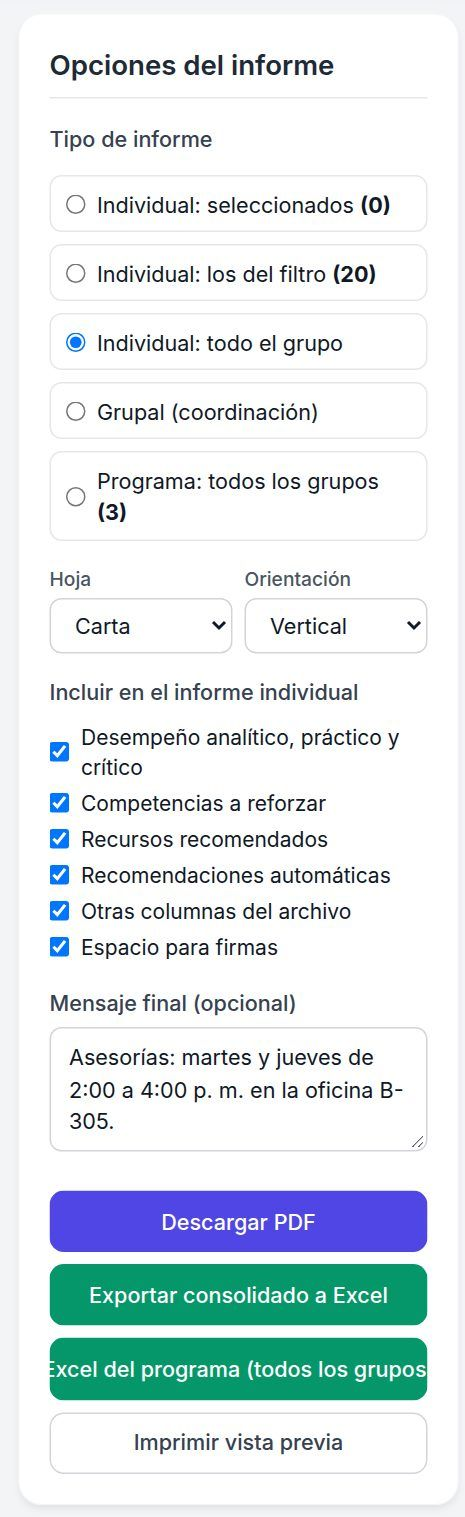
\includegraphics[width=0.97\linewidth]{img/informes_opciones.jpg}}}
\end{minipage}\hfill
\begin{minipage}[t]{0.73\linewidth}\vspace{0pt}\centering
{\setlength{\fboxsep}{0pt}\fcolorbox{gris!35}{white}{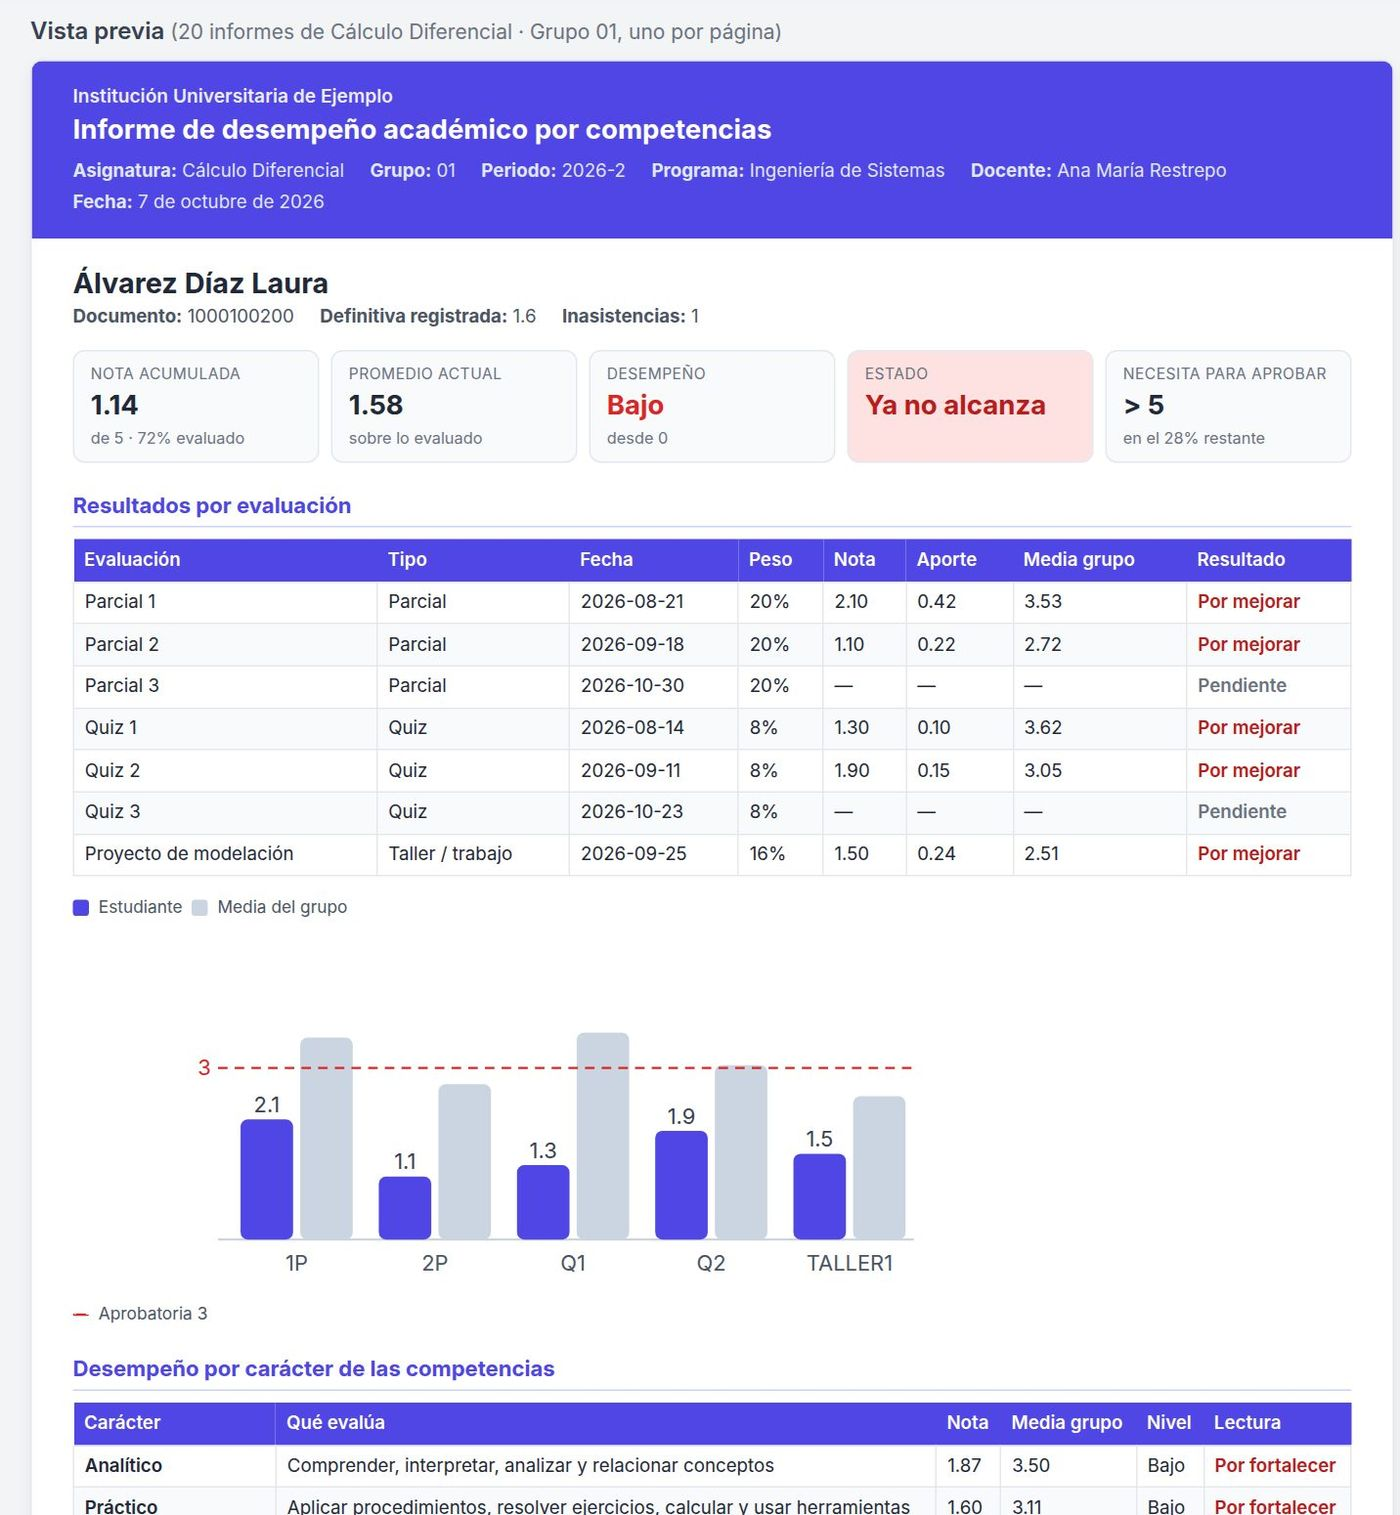
\includegraphics[width=0.99\linewidth]{img/informes_vista.jpg}}}
\end{minipage}
\caption{Opciones del informe (izquierda) y vista previa (derecha).}\label{fig:informes}
\end{figure}

\section{Tipos de informe}\label{sec:tiposinf}
\begin{tabularx}{\linewidth}{>{\bfseries}l X}
\toprule
Individual: seleccionados & Un informe por página para los estudiantes marcados (\ver{sec:seleccion}).\\
Individual: los del filtro & Para los que cumplen el filtro de la pestaña 4 (\ver{sec:criterios}).\\
Individual: todo el grupo & Para todos los estudiantes del grupo activo.\\
Grupal & Informe del grupo activo para el docente o la coordinación.\\
Programa & Informe global de todos los grupos (\ver{sec:infprog}).\\
\bottomrule
\end{tabularx}

\section{Opciones}\label{sec:opcionesinf}
\begin{itemize}
  \item \textbf{Hoja} (carta, oficio, A4) y \textbf{orientación}. El informe del programa siempre sale horizontal.
  \item \textbf{Incluir en el informe individual}: desempeño analítico, práctico y crítico; competencias a reforzar; recursos recomendados; recomendaciones automáticas; otras columnas del archivo; espacio para firmas.
  \item \textbf{Mensaje final}: por ejemplo el horario de asesorías.
\end{itemize}

\section{Contenido de cada informe}\label{sec:contenidoinf}
\begin{description}[style=nextline,leftmargin=1.2em,font=\color{primario}\bfseries]
  \item[Individual] Encabezado del curso; datos del estudiante; indicadores (acumulado, promedio, desempeño, estado, nota necesaria); tabla por evaluación con la media del grupo; gráfico; \textbf{desempeño por carácter} con lectura «Fortaleza / Logrado / Por fortalecer»; competencias a reforzar (hasta 12, las comprometidas en más evaluaciones); recursos con enlaces activos; recomendaciones; observaciones; firmas.
  \item[Grupal] Indicadores; cuatro gráficos; desempeño por carácter; estadísticas por evaluación; estudiantes en riesgo; logro por competencia; competencias críticas; mejores promedios; consolidado de notas.
  \item[Programa] Ver \ver{sec:infprog}.
\end{description}

\section{PDF, Excel e impresión}\label{sec:exportar}
\begin{itemize}
  \item \ui{Descargar PDF}: genera el PDF del tipo elegido, con texto real (se puede buscar y copiar) y enlaces activos.
  \item \ui{Exportar consolidado a Excel}: libro del grupo activo con las hojas \emph{Consolidado} (incluye notas por carácter), \emph{Estadísticas}, \emph{Competencias críticas}, \emph{Plan por estudiante} y \emph{Configuración}.
  \item \ui{Excel del programa (todos los grupos)}: ver \ver{sec:infprog}.
  \item \ui{Imprimir vista previa}: imprime solo los informes mostrados (máximo 8 en la vista previa; el PDF incluye todos).
\end{itemize}

\navegacion{cap:estudiantes}{cap:programa}

% =====================================================================
\chapter{Pestaña 6 · Programa (todos los grupos)}\label{cap:programa}
\enestecapitulo
Esta pestaña junta a todos los estudiantes de todos los grupos cargados. Sirve para la coordinación del programa, el comité curricular o el docente que tiene varios grupos.

\section{Indicadores globales}\label{sec:kpisprog}
\captura{programa_kpis.jpg}{Indicadores del programa.}{kpisprog}
Grupos y docentes, estudiantes, promedio del programa, cuántos van aprobando, cuántos están en riesgo o perdiendo y la \textbf{brecha entre grupos} (diferencia entre el mejor promedio y el más bajo, \ver{sec:indprog}).

\section{Desempeño por carácter en el programa}\label{sec:dimprog}
\captura{programa_caracter.jpg}{Carácter de las competencias en todo el programa y en cada grupo.}{dimprog}
\begin{itemize}
  \item Tres tarjetas con la media, el logro, las competencias evaluadas y el porcentaje del peso de cada carácter.
  \item \textbf{Media por carácter en cada grupo}: barras azules (analítico), verdes (práctico) y moradas (crítico) por grupo, con la línea de la aprobatoria.
  \item \textbf{Promedio actual por grupo}: en naranja, los grupos por debajo de la aprobatoria.
\end{itemize}

\section{Hallazgos y recomendaciones}\label{sec:hallazgos}
\captura{programa_hallazgos.jpg}{Hallazgos y recomendaciones generados a partir de los datos.}{hallazgos}
Los \textbf{hallazgos} resumen la situación: carácter más débil y más fuerte, participación de cada carácter en el peso de las evaluaciones, brecha entre grupos, grupos por debajo de la aprobatoria, competencias y evaluación con menor logro, estudiantes sin notas.

Las \textbf{recomendaciones} proponen acciones: fortalecer el carácter más débil, evaluar más el pensamiento crítico si pesa menos del 15\,\%, acompañar a los estudiantes en riesgo, reducir la brecha entre grupos y reforzar competencias comunes. Ver también \ver{tarea:critico}.

\section{Comparativo de grupos y resumen por curso}\label{sec:comparativo}
\captura{programa_grupos.jpg}{Comparativo de grupos.}{comparativo}
Para cada grupo: docente, curso, estudiantes, porcentaje evaluado, promedio, porcentaje aprobando, en riesgo, no alcanzan y la media de cada carácter (entre paréntesis, el logro). \textbf{Haga clic en un grupo} para activarlo y ver su análisis en la pestaña 3. Si hay grupos de varios cursos aparece además el resumen \textbf{por curso}.

\section{Competencias y evaluaciones del programa}\label{sec:compprog}
\captura{programa_competencias.jpg}{Competencias del programa y evaluaciones con menor aprobación.}{compprog}
\begin{itemize}
  \item \textbf{Competencias del programa}: logro de cada competencia sumando todos los grupos. Filtre por carácter y ordene por menor o mayor logro.
  \item \textbf{Evaluaciones con menor aprobación}: las evaluaciones de todos los grupos ordenadas por su porcentaje de aprobación.
\end{itemize}

\section{Estudiantes en riesgo en todo el programa}\label{sec:riesgoprog}
\captura{programa_riesgo.jpg}{Estudiantes con alerta en todos los grupos.}{riesgoprog}
Busque por nombre o grupo y filtre por estado. Haga clic en un nombre para abrir su ficha; la aplicación activa su grupo automáticamente.

\section{Informes del programa}\label{sec:infprog}
\begin{itemize}
  \item \ui{Informe PDF del programa}: hoja horizontal con indicadores, hallazgos, carácter, gráficos, comparativo de grupos, por curso, competencias con menor y mayor logro, evaluaciones críticas, recomendaciones y estudiantes en riesgo.
  \item \ui{Excel del programa}: hojas \emph{Resumen}, \emph{Grupos}, \emph{Por curso}, \emph{Competencias}, \emph{Evaluaciones}, \emph{Estudiantes} (todos, con su grupo y notas por carácter) y \emph{Clasificación} (carácter de cada competencia de los cursos en uso, automático y corregido).
  \item \ui{Carácter de las competencias}: abre la ventana de corrección (\ver{sec:corregir}).
\end{itemize}

\navegacion{cap:informes}{cap:caracter}

% =====================================================================
\chapter{Carácter de las competencias}\label{cap:caracter}
\enestecapitulo

\section{Las tres dimensiones}\label{sec:tresdim}
\begin{tcbraster}[raster columns=3,raster equal height,enhanced,arc=3pt,fontupper=\small,fonttitle=\bfseries\sffamily]
\begin{tcolorbox}[colframe=analitico,colback=analitico!6,title={Analítico}]
Comprender, interpretar, analizar y relacionar conceptos. \emph{Ejemplo: «Analizar la continuidad de una función».}
\end{tcolorbox}
\begin{tcolorbox}[colframe=practico,colback=practico!6,title={Práctico}]
Aplicar procedimientos, resolver ejercicios, calcular y usar herramientas. \emph{Ejemplo: «Aplicar la regla de la cadena».}
\end{tcolorbox}
\begin{tcolorbox}[colframe=critico,colback=critico!6,title={Pensamiento crítico}]
Evaluar, argumentar, justificar, modelar y decidir ante problemas. \emph{Ejemplo: «Formular y resolver modelos de optimización en situaciones reales».}
\end{tcolorbox}
\end{tcbraster}

\section{Clasificación automática}\label{sec:clasificacion}
Cada competencia del catálogo se clasifica al cargarlo:
\begin{pasos}
  \item El \textbf{verbo inicial} suma 3 puntos a su carácter (si empieza con dos verbos, «Comprender y aplicar…», el segundo suma 2).
  \item Cada \textbf{palabra clave} del texto o del criterio suma 1 punto (por ejemplo «interpretación», «aplicación», «justificación»).
  \item «Resolver \textbf{problemas}» en contexto (optimización, modelación, situaciones reales, física, economía, ingeniería…) suma 3 puntos a pensamiento crítico.
  \item «Evaluar integrales / límites / expresiones» se toma como práctico (es calcular).
  \item Gana el carácter con más puntos; en empate, el del verbo inicial.
\end{pasos}

\begin{longtable}{>{\raggedright\arraybackslash}p{2.6cm}>{\raggedright\arraybackslash}p{12.8cm}}
\toprule
\textbf{Carácter} & \textbf{Verbos iniciales reconocidos}\\\midrule\endhead
\dimA & comprender, analizar, identificar, interpretar, estudiar, determinar, describir, representar, comparar, establecer, reconocer, distinguir, explicar, clasificar, relacionar, examinar, demostrar, deducir, definir, caracterizar, visualizar, conocer, entender, estimar, observar, abstraer\\
\dimP & resolver, aplicar, utilizar, usar, calcular, implementar, desarrollar, trabajar, emplear, simplificar, construir, manejar, operar, factorizar, manipular, documentar, desplegar, entrenar, realizar, configurar, ejecutar, programar, graficar, trazar, derivar, integrar, expresar, convertir, medir, elaborar, codificar, hallar, encontrar, efectuar, practicar\\
\dimC & evaluar, valorar, validar, justificar, argumentar, juzgar, criticar, optimizar, diseñar, crear, modelar, formular, plantear, proponer, decidir, seleccionar, elegir, contrastar, verificar, reflexionar, cuestionar, debatir, inferir, sintetizar, concluir, generalizar, investigar, innovar\\
\bottomrule
\end{longtable}

\section{Revisar y corregir la clasificación}\label{sec:corregir}
\captura[0.85\linewidth]{modal_caracter.jpg}{Ventana «Carácter de las competencias».}{modalcaracter}
\begin{pasos}
  \item Ábrala con \ui{Revisar el carácter de las competencias} (pestaña 1) o \ui{Carácter de las competencias} (pestaña 6).
  \item Elija el curso (los que están en uso aparecen primero), filtre por carácter o busque.
  \item Cambie el carácter en la lista de la derecha. La opción marcada «(automático)» es la clasificación original.
  \item Las competencias corregidas muestran «Corregida (automática: …)». \ui{Volver a la clasificación automática} quita las correcciones del curso.
\end{pasos}
El cambio se aplica a todos los grupos y se recalcula todo al instante. Se conserva aunque vuelva a cargar el catálogo.

\section{De la competencia a la nota por carácter}\label{sec:dimnota}
\begin{enumerate}
  \item \textbf{Perfil de cada evaluación}: proporción de sus competencias de cada carácter. Si 1P mide 2 competencias analíticas y 1 práctica, su perfil es 67\,\% analítico y 33\,\% práctico. Si el docente fijó el carácter, es 100\,\% de ese carácter (\ver{sec:caracterev}).
  \item \textbf{Nota del estudiante en el carácter $k$}: promedio de sus notas en las evaluaciones calificadas, ponderado por el peso $p_i$ de cada evaluación y la proporción $w_{ik}$ de ese carácter:
  \[ N_k = \frac{\sum_i n_i\, p_i\, w_{ik}}{\sum_i p_i\, w_{ik}} \]
  Las evaluaciones sin presentar cuentan como 0 si así está configurado (\ver{sec:escala}); las pendientes no cuentan.
  \item \textbf{Grupo y programa}: la media de las notas $N_k$ de los estudiantes y el \textbf{logro}, el porcentaje de estudiantes con $N_k \geq$ aprobatoria.
\end{enumerate}

\section{Cómo interpretar los resultados}\label{sec:interpretar}
\begin{itemize}
  \item Compare los tres caracteres: una diferencia grande indica dónde concentrar el refuerzo.
  \item Mire también el \textbf{porcentaje del peso}: si el pensamiento crítico pesa poco o nada, el resultado dice poco sobre él y conviene evaluarlo más (\ver{tarea:critico}).
  \item Un carácter con pocas competencias evaluadas es menos confiable.
  \item En el informe individual, «Por fortalecer» indica una nota por debajo de la aprobatoria; «Fortaleza», una nota aprobatoria y mayor o igual a la media del grupo.
\end{itemize}
\begin{atencion}
La clasificación automática es una ayuda, no un juicio pedagógico definitivo. Revise sobre todo las competencias de los cursos que está analizando.
\end{atencion}

\navegacion{cap:programa}{cap:calculos}

% =====================================================================
\chapter{Cómo se calcula}\label{cap:calculos}
\enestecapitulo

\section{Evaluaciones calificadas, pendientes y sin presentar}\label{sec:pendientes}
\begin{itemize}
  \item \textbf{Calificada}: al menos un estudiante del grupo tiene nota.
  \item \textbf{Pendiente}: nadie tiene nota todavía; cuenta para lo que falta por evaluar.
  \item \textbf{Sin presentar}: la evaluación está calificada pero el estudiante no tiene nota (celda vacía o \col{NP}). Cuenta como 0 si la opción está marcada (\ver{sec:escala}).
\end{itemize}

\section{Nota acumulada, promedio y nota necesaria}\label{sec:formulas}
Con $n_i$ la nota y $p_i$ el peso (\%) de cada evaluación, $P_{\text{eval}}$ el porcentaje evaluado, $P_{\text{rest}}$ el que falta, $P$ el total y $a$ la nota aprobatoria:
\begin{align*}
\text{Acumulado } A &= \sum_{\text{calificadas}} \frac{n_i\,p_i}{100} &
\text{Promedio actual} &= \frac{A}{P_{\text{eval}}/100}\\[4pt]
\text{Nota necesaria} &= \frac{a\,P/100 - A}{P_{\text{rest}}/100} &
\text{Máximo posible} &= A + \frac{\text{nota máxima}\cdot P_{\text{rest}}}{100}
\end{align*}
\begin{nota}
Ejemplo: con 1P = 3.1, 2P = 3.0 y 3P = 2.0 (20\,\% cada uno) y Q1 = 1.0, Q2 = 4.0, Q3 = 3.0 (5\,\% cada uno), el acumulado es 2.02, el promedio 2.69 y, faltando 25\,\%, necesita 3.92.
\end{nota}

\section{Estados académicos}\label{sec:estados}
\begin{tabularx}{\linewidth}{>{\bfseries}l X}
\toprule
\textcolor{verde}{Aprobado} & Periodo cerrado y nota final $\geq$ aprobatoria.\\
\textcolor{verde}{Aprobación asegurada} & El acumulado ya alcanza la aprobatoria aunque falten evaluaciones.\\
\textcolor{azul}{Va aprobando} & Promedio actual $\geq$ aprobatoria.\\
\textcolor{ambar}{En riesgo} & Promedio por debajo de la aprobatoria; necesita una nota alcanzable.\\
\textcolor{ambar}{Riesgo alto} & Necesita más que el umbral (por defecto 4.0) en lo que falta.\\
\textcolor{rojo}{Ya no alcanza} & Ni con la nota máxima en lo que falta llega a la aprobatoria.\\
\textcolor{rojo}{Reprobado} & Periodo cerrado y nota final por debajo de la aprobatoria.\\
\textcolor{gris}{Sin calificaciones} & No tiene ninguna nota registrada.\\
\bottomrule
\end{tabularx}

\section{Niveles de desempeño}\label{sec:niveles}
Según el promedio actual: \textbf{Superior} $\geq$ 4.6, \textbf{Alto} $\geq$ 4.0, \textbf{Básico} $\geq$ 3.0 y \textbf{Bajo}. Los nombres y límites se cambian en \ver{sec:escala}.

\section{Tendencia}\label{sec:tendencia}
Compara el último parcial con el promedio de los parciales anteriores (si hay menos de dos parciales, todas las notas en orden). Una diferencia mayor que 0.3 es \emph{mejora} o \emph{baja}; si no, \emph{estable}.

\section{Indicadores del programa}\label{sec:indprog}
\begin{itemize}
  \item \textbf{Promedio del programa}: media de los promedios de todos los estudiantes con notas.
  \item \textbf{Brecha}: promedio del mejor grupo menos el del grupo más bajo; desde 0.5 se considera significativa.
  \item \textbf{Logro de una competencia}: porcentaje de estudiantes de todos los grupos que la miden cuya nota en sus evaluaciones (ponderada por peso) alcanza la aprobatoria.
  \item \textbf{Participación de un carácter}: parte del peso de las evaluaciones que le corresponde, promediada entre grupos.
\end{itemize}

\navegacion{cap:caracter}{cap:respaldo}

% =====================================================================
\chapter{Guardar, respaldos y empezar de nuevo}\label{cap:respaldo}
\enestecapitulo

\section{Guardado automático}\label{sec:autoguardado}
Cada cambio se guarda solo en el navegador. Al volver a abrir \texttt{index.html} en el \textbf{mismo navegador y computador}, el trabajo sigue ahí, con todos los grupos.

\section{Respaldo}\label{sec:respaldo}
\begin{itemize}
  \item \ui{Guardar respaldo} descarga un archivo \texttt{.json} con todo: grupos, notas, porcentajes, competencias, carácter corregido, observaciones y opciones.
  \item \ui{Abrir respaldo} lo recupera en cualquier computador. También abre los respaldos de la versión 3 (un solo grupo).
\end{itemize}
\begin{consejo}
Guarde un respaldo al terminar cada sesión y antes de borrar los datos del navegador o cambiar de computador.
\end{consejo}

\section{Empezar de nuevo}\label{sec:nuevo}
\ui{Nuevo} borra todos los grupos, el catálogo y la configuración (pide confirmación). Para quitar un solo grupo use la \ui{\textcolor{rojo}{x}} de la lista de grupos (\ver{sec:listagrupos}).

\section{Privacidad}\label{sec:privacidad}
Los archivos se leen en su navegador; ningún dato se envía a internet. Solo se descargan las librerías de Excel y PDF. Los enlaces de recursos llevan a sitios externos únicamente cuando alguien hace clic en ellos.

\navegacion{cap:calculos}{cap:manual}

% =====================================================================
\chapter{Pestaña 7 · Manual y ayuda}\label{cap:manual}
\enestecapitulo

\section{El manual dentro de la aplicación}\label{sec:pestanamanual}
\begin{itemize}
  \item A la izquierda, el \textbf{índice} con todos los capítulos y secciones y su página. Haga clic para ir.
  \item \ui{Buscar tema}: filtra el índice por palabras.
  \item \ui{‹ Tema anterior} y \ui{Tema siguiente ›} recorren los temas en orden.
  \item \ui{Abrir en otra pestaña} y \ui{Descargar el PDF}.
  \item Dentro del PDF funcionan todos los enlaces: mapa rápido, índice, cabeceras y referencias.
\end{itemize}

\section{El botón Ayuda}\label{sec:botonayuda}
\ui{? Ayuda}, en la cabecera, abre este manual en el capítulo de la pestaña que usted está usando: por ejemplo, desde la pestaña 4 abre \ver{cap:estudiantes}.

\navegacion{cap:respaldo}{cap:tareas}

% =====================================================================
\chapter{Tareas frecuentes paso a paso}\label{cap:tareas}
\enestecapitulo

\section{Analizar un grupo por primera vez}\label{tarea:ungrupo}
\begin{pasos}
  \item Abra \texttt{index.html}. En \pest{cap:datos}{1. Datos} cargue la planilla del grupo (\ver{sec:cargarnotas}).
  \item Cargue el catálogo de competencias y elija el curso (\ver{sec:cargarcatalogo}).
  \item Complete institución, asignatura, grupo, periodo y docente (\ver{sec:datosgrupo}).
  \item En \pest{cap:evaluaciones}{2. Evaluaciones} revise que los porcentajes sumen 100\,\% y agregue las fechas (\ver{sec:pesos}).
  \item Revise las competencias de cada evaluación (\ver{sec:asociar}).
  \item Mire \pest{cap:analisis}{3. Análisis} y las alertas (\ver{sec:alertas}).
  \item Guarde un respaldo (\ver{sec:respaldo}).
\end{pasos}

\section{Analizar varios grupos de un programa}\label{tarea:varios}
\begin{pasos}
  \item Reúna las planillas: un archivo por grupo, una hoja por grupo o una hoja con columna \col{Grupo} (\ver{sec:variosgrupos}).
  \item En \pest{cap:datos}{1. Datos} selecciónelas todas juntas.
  \item Cargue el catálogo y revise el curso de cada grupo en la lista; cambie los nombres de los grupos si lo desea (\ver{sec:listagrupos}).
  \item Configure las evaluaciones de un grupo y use \ui{Copiar a los demás grupos} (\ver{sec:copiar}).
  \item Revise la clasificación de las competencias de los cursos en uso (\ver{sec:corregir}).
  \item Abra \pest{cap:programa}{6. Programa}: revise hallazgos, comparativo y competencias.
  \item Descargue el PDF y el Excel del programa (\ver{sec:infprog}).
\end{pasos}

\section{Informes para estudiantes en riesgo}\label{tarea:riesgo}
\begin{pasos}
  \item En \pest{cap:estudiantes}{4. Estudiantes} use el filtro rápido \emph{En riesgo, perdiendo o sin notas} (\ver{sec:rapidos}).
  \item Abra la ficha de cada uno y escriba observaciones (\ver{sec:ficha}).
  \item En \pest{cap:evaluaciones}{2. Evaluaciones} agregue recursos a las evaluaciones perdidas (\ver{sec:recursos}).
  \item En \pest{cap:informes}{5. Informes} elija \emph{Individual: los del filtro}, escriba el mensaje final con el horario de asesorías y descargue el PDF.
\end{pasos}

\section{Informe para coordinación o comité}\label{tarea:coordinacion}
\begin{pasos}
  \item Para un grupo: \pest{cap:informes}{5. Informes} $\rightarrow$ \emph{Grupal} $\rightarrow$ \ui{Descargar PDF} y \ui{Exportar consolidado a Excel}.
  \item Para todo el programa: \pest{cap:programa}{6. Programa} $\rightarrow$ \ui{Informe PDF del programa} y \ui{Excel del programa}.
  \item Complemente con los hallazgos y recomendaciones (\ver{sec:hallazgos}).
\end{pasos}

\section{Fortalecer el pensamiento crítico}\label{tarea:critico}
\begin{pasos}
  \item En \pest{cap:programa}{6. Programa} mire la tarjeta de \dimC: su media, su logro y \textbf{qué parte del peso} tiene (\ver{sec:dimprog}).
  \item Si pesa poco o nada, incluya en las próximas evaluaciones problemas abiertos, estudios de caso, proyectos o preguntas de justificación.
  \item Asocie a esas evaluaciones competencias de modelación, validación o argumentación, o fije su carácter como \dimC\ (\ver{sec:caracterev}).
  \item Revise que las competencias del curso estén bien clasificadas (\ver{sec:corregir}).
  \item Siga el avance comparando el logro por carácter a lo largo del semestre.
\end{pasos}

\section{Actualizar notas a mitad del semestre}\label{tarea:actualizar}
\begin{pasos}
  \item Actualice las notas en su Excel o CSV (sin cambiar los encabezados).
  \item Vuelva a cargarlo en \pest{cap:datos}{1. Datos}: los grupos de ese archivo se actualizan y conservan porcentajes, fechas, competencias, carácter y observaciones (\ver{sec:variosgrupos}).
  \item Si agregó una evaluación nueva (por ejemplo 4P), revise los porcentajes (\ver{sec:pesos}).
\end{pasos}

\navegacion{cap:manual}{cap:problemas}

% =====================================================================
\chapter{Solución de problemas}\label{cap:problemas}
\enestecapitulo

\section{Al cargar archivos}\label{sec:problemascarga}
\begin{description}[style=nextline,leftmargin=1.2em,font=\color{primario}\bfseries]
  \item[«No se encontró la columna de nombres»] La hoja debe tener un encabezado como \col{Nombres y Apellidos} o \col{Estudiante} en las primeras 20 filas (\ver{sec:planilla}).
  \item[Una columna de notas se leyó como texto o como dato informativo] Tiene sobre todo texto, o valores fuera de la escala. Revise «Observaciones de la lectura» (\ver{sec:cargarnotas}) y la escala (\ver{sec:escala}).
  \item[Las tildes del CSV se ven mal] Guarde el CSV como «CSV UTF-8» desde Excel; la aplicación también reconoce el formato de Excel en español (\ver{sec:csv}).
  \item[Se crearon grupos que no esperaba] La hoja tiene una columna \col{Grupo}, \col{Asignatura} o \col{Curso} con varios valores (\ver{sec:variosgrupos}). Quite los grupos sobrantes con la \ui{\textcolor{rojo}{x}}.
  \item[El curso de competencias no es el correcto] Cámbielo en la lista de grupos (\ver{sec:listagrupos}).
\end{description}

\section{En el análisis}\label{sec:problemasanalisis}
\begin{description}[style=nextline,leftmargin=1.2em,font=\color{primario}\bfseries]
  \item[«Los porcentajes suman \ldots\ (deberían sumar 100\,\%)»] Ajústelos o use \ui{Repartir porcentajes} (\ver{sec:pesos}).
  \item[No aparece el análisis por carácter] Las evaluaciones no tienen competencias ni carácter fijado (\ver{sec:asociar} y \ver{sec:caracterev}).
  \item[Pensamiento crítico aparece sin datos] Ninguna evaluación calificada mide competencias de ese carácter (\ver{sec:interpretar}).
  \item[Un estudiante tiene 0 donde no presentó] Es la opción «celda vacía cuenta como 0» (\ver{sec:escala}).
\end{description}

\section{Informes y almacenamiento}\label{sec:problemasinformes}
\begin{description}[style=nextline,leftmargin=1.2em,font=\color{primario}\bfseries]
  \item[«Librerías sin cargar»] Conéctese a internet y recargue la página (F5) (\ver{sec:requisitos}).
  \item[El PDF no muestra a todos los estudiantes en la vista previa] La vista previa muestra hasta 8; el PDF los incluye todos (\ver{sec:exportar}).
  \item[Perdí mis datos] Los datos están en el navegador donde trabajó. Use \ui{Abrir respaldo} con su último \texttt{.json} (\ver{sec:respaldo}).
  \item[El manual no se ve en la pestaña 7] Use \ui{Abrir en otra pestaña} o \ui{Descargar el PDF} (\ver{cap:manual}).
\end{description}

\navegacion{cap:tareas}{cap:glosario}

% =====================================================================
\chapter{Glosario}\label{cap:glosario}
Haga clic en el término entre paréntesis para ir a su explicación.

\begin{description}[style=nextline,leftmargin=1.2em,font=\color{primario}\bfseries,itemsep=3pt]
  \item[Acumulado] Lo ganado hasta hoy sobre la nota final (\ver{sec:formulas}).
  \item[Alerta temprana] Estudiante en riesgo, que ya no alcanza o sin notas (\ver{sec:alertas}).
  \item[Analítico] Carácter de comprender, interpretar y analizar (\ver{sec:tresdim}).
  \item[Brecha entre grupos] Diferencia entre el mejor y el peor promedio de grupo (\ver{sec:indprog}).
  \item[Carácter] Dimensión de una competencia o evaluación: analítico, práctico o crítico (\ver{cap:caracter}).
  \item[Catálogo de competencias] Excel con las competencias de cada curso (\ver{sec:catalogo}).
  \item[Competencia crítica] Competencia con bajo logro en el grupo o en el programa (\ver{sec:alertas}).
  \item[Criterio de filtro] Condición sobre un campo para mostrar estudiantes (\ver{sec:criterios}).
  \item[Estado académico] Situación del estudiante: va aprobando, en riesgo, ya no alcanza… (\ver{sec:estados}).
  \item[Evaluación pendiente] Evaluación que nadie ha presentado aún (\ver{sec:pendientes}).
  \item[Grupo activo] Grupo que muestran las pestañas 2 a 5 (\ver{sec:listagrupos}).
  \item[Logro] Porcentaje de estudiantes que alcanzan la aprobatoria (\ver{sec:dimnota}).
  \item[Nivel de desempeño] Superior, Alto, Básico o Bajo según el promedio (\ver{sec:niveles}).
  \item[Nota necesaria] Promedio que necesita en lo que falta para aprobar (\ver{sec:formulas}).
  \item[NP] No presentó (\ver{sec:pendientes}).
  \item[Pensamiento crítico] Carácter de evaluar, justificar, modelar y decidir (\ver{sec:tresdim}).
  \item[Perfil de la evaluación] Proporción de cada carácter en una evaluación (\ver{sec:dimnota}).
  \item[Peso] Porcentaje de la nota final que vale una evaluación (\ver{sec:pesos}).
  \item[Práctico] Carácter de aplicar, resolver y calcular (\ver{sec:tresdim}).
  \item[Programa] Conjunto de todos los grupos cargados (\ver{cap:programa}).
  \item[Promedio actual] Nota que lleva sobre lo evaluado (\ver{sec:formulas}).
  \item[Recursos] Páginas, videos, ejercicios y herramientas recomendados (\ver{sec:recursos}).
  \item[Respaldo] Archivo .json con todo el trabajo (\ver{sec:respaldo}).
  \item[Tendencia] Mejora o baja entre los últimos parciales (\ver{sec:tendencia}).
\end{description}

\navegacion{cap:problemas}{}

\end{document}
